\chapter[Análisis de Requisitos]{Análisis de Requisitos globales}

En este capítulo explicaremos el proceso de análisis de requisitos llevado a cabo para la elaboración de la aplicación y toda la información recibida por la comunidad, así como las decisiones tomadas en base a la experiencia de otros proyectos similares al nuestro.

\section{Consultas con la comunidad}

A la hora de realizar las consultas con la comunidad hemos decidido contactar con la sede local de la ONCE para recabar información sobre las dificultades que los invidentes se encuentran a la hora de utilizar diferentes dispositivos y programas informáticos.
También hemos preguntado a personas daltónicas para que nos aconsejarán desde su experiencia sobre cómo se deberían realizar juegos sin que ellos se vean afectados por su diseño.

Ambas consultas, así como el resultado obtenido de las mismas, se detallaron en la Sección~\ref{sec:dificultadesfeedback} 

\subsection{Resumen de las peticiones recibidas}
	\paragraph{Posibilidad de cambiar el color de la interfaz} La interfaz gráfica tendrá diferentes colores que diferencien los distintos tipos de enemigos y elementos del juego de cara a los jugadores videntes. Tal y como se menciona en la Sección~\ref{sec:solventadodaltonicos}, debemos tener en cuenta específicamente el caso de los usuarios daltónicos a pesar de que dichos elementos son fácilmente diferenciables.
	\paragraph{Variedad en las descripciones automáticas de los elementos del juego} Las personas invidentes necesitan tener un \textit{feedback} auditivo para saber qué es lo que está sucediendo y así poder tomar una decisión razonada en base a la situación en la que se encuentran. Debemos generar estas descripciones de la forma más variada y correcta posible para que no sean repetitivas. 
	\paragraph{Diferentes idiomas} Al ser un videojuego en el cual el lenguaje es esencial, debemos tener en cuenta la posibilidad de incluir otros idiomas.
  \paragraph{Utilizar el idioma en nuestro favor} Usar elementos de temporalidad o diferentes adjetivos para definir ciertos elementos para que el lenguaje sea parte de la experiencia.
	\paragraph{Multiplataforma} Tal y como mencionamos en la introducción, nuestro software debe poder ser ejecutado en varios sistemas operativos (Linux, Mac OS, Windows...).
	
\subsection{Cómo hemos abordado el problema de accesibilidad para invidentes en nuestro proyecto}

En el proyecto hemos creado descripciones para todos los elementos de la pantalla, por lo que el jugador siempre puede saber dónde se encuentra, qué hay a su alrededor, cuáles son sus características, las del enemigo y las de los elementos equipables, etc. También hemos creado una ventana que se encuentra al lado del juego y donde se van guardando de forma ordenada todas las frases generadas, siendo la primera de ellas la última generada y leyéndose automáticamente por el reproductor de pantalla que esté siendo usado en ese momento (en nuestro caso, \textit{NVDA}). De esta forma, una persona con visión siempre puede leer dicha frase mientras que el jugador invidente puede volver a escucharla las veces que quiera. Además, dicho listado funciona a modo de \textit{log}, por lo que el jugador también puede recordar lo sucedido anteriormente gracias a que estos mensajes permanecen disponibles en la pantalla y pueden ser leidos por el software lector. La Figura \ref{fig:roomsgametextarea} muestra la captura de pantalla de esta ventana para una sesión de juego.

\begin{figure}[H]
		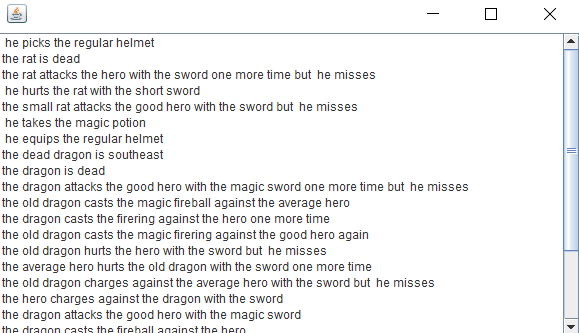
\includegraphics[width=\textwidth,height=\textheight,keepaspectratio]{./img/roomsGameTextArea.png}
	\caption{Captura de pantalla del área donde mostramos las frases generadas por nuestro juego para invidentes}
	\label{fig:roomsgametextarea}
\end{figure}

\subsection{Cómo hemos abordado el problema de accesibilidad para daltónicos en nuestro proyecto}
\label{sec:solventadodaltonicos}

En nuestro caso, al haber preguntado de antemano a los potenciales usuarios, siempre tuvimos la idea de crear la interfaz gráfica con soporte para daltónicos en mente.

De este modo, todos los elementos del juego que se encuentran en la interfaz gráfica son distinguibles entre sí gracias al uso de caracteres completamente diferentes por lo que, incluso aunque todos los colores fueran iguales, sería sencillo identificar cada elemento sólo por su forma en vez de por su color. 

De todas maneras, hemos creado una opción que cambia la paleta de colores a utilizar y facilita su visualización para aquellos usuarios que sufren daltonismo.

\section{Análisis de los elementos del juego}
Al ser un \textit{roguelike}, debemos incluir los elementos característicos del género: aleatoriedad, dificultad, progreso, etc. Los detalles acerca de los mismos, así como la forma en la que han sido introducidos en el proyecto han sido ya comentados en la Sección~\ref{sec:roguelikeinformacion}.

\section{Requisitos del aplicativo}
Con toda la información obtenida y analizada, creamos una lista con los casos de uso que nuestro proyecto debe cumplir y cuyo diagrama mostramos en la Figura \ref{fig:roomsgametextarea}:

\begin{itemize}
  \item \textbf{Movimiento} Un usuario siempre será capaz de moverse con su personaje a una posición válida dentro de la habitación donde se encuentra. 
  \item \textbf{Ataque normal} Cuando el personaje está en la misma posición que un enemigo, éste será capaz de atacar cuerpo a cuerpo.
  \item \textbf{Ataque mágico} Cuando el personaje está dentro de una distancia determinada de un enemigo, aquél será capaz de realizar un ataque mágico, siempre y cuando tenga sufiencience maná para el mismo. Si el enemigo se encuentra demasiado lejos, el ataque mágico se realizará, pero sin afectar a ningún enemigo (por lo que el usuario perderá maná).
  \item \textbf{Coger elemento} En las habitaciones del mapa habrá elementos que se pueden recolectar, así como enemigos que soltarán diferentes objetos.
  \item \textbf{Equipar elemento} Poder equipar a nuestro personaje con un objeto que está en el inventario, siempre y cuando no tengamos un objeto del mismo tipo ya equipado.
  \item \textbf{Desequipar elemento} De la misma manera, podremos desequipar un objeto que tenemos equipado mientras tengamos espacio en el inventario.
  \item \textbf{Tirar elemento} En algunas ocasiones el jugador podría encontrarse con que no dispone de espacio suficiente en el inventario para almacenar nuevos elementos, por lo que podrá arrojar objetos al suelo para hacer hueco a aquellos nuevos que queramos recoger.
  \item \textbf{Descripciones} Durante el transcurso del juego podremos generar diferentes descripciones de lo que ocurre en el juego dependiendo de lo que queramos saber. Por ejemplo: lo que el personaje del jugador tiene en el inventario, las posiciones a las que nos podemos mover, la descripciones de los enemigos a los que nos enfrentamos, las estadísticas del héroe y de los enemigos, etc.
  \item \textbf{Activación de descripciones numéricas} Algunas de estas descripciones corresponden a posiciones o características de los enemigos que el usuario podría querer escuchar como valor numérico (por ejemplo la cantidad de vida de un monstruo) o mediante expresiones del lenguage (``mucha'', ``poca'', ``bastante'', etc.), dependiendo de lo que prefiera.
  \item \textbf{Cambio de colores} Para usuarios daltónicos hemos incluido una opción para cambiar los colores de la interfaz gráfica.
\end{itemize}

\noindent Asimismo, al realizar algunas de estas acciones (coger, equipar, desequipar y tirar un objeto, moverse y atacar), un turno será consumido. Al consumir el jugador su turno, pasará entonces el turno a los enemigos, que realizarán sus acciones como, or ejemplo, acercarse o atacar al jugador.

\begin{figure}[h!]
    \centering
    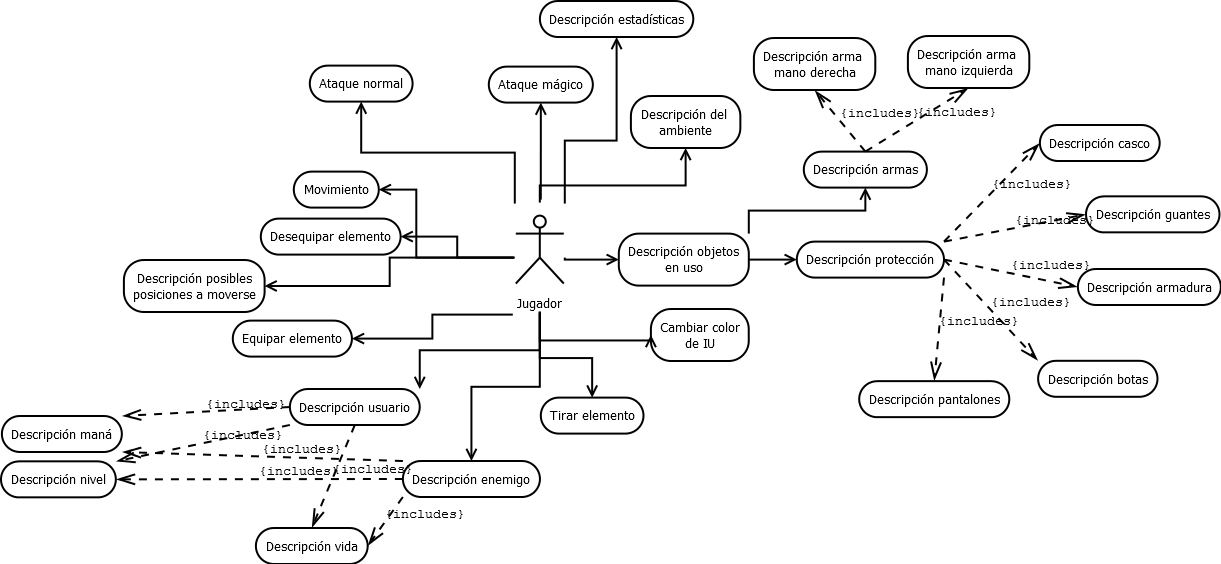
\includegraphics[width=0.9\textheight,angle=90]{img/casosdeuso.png}
    \caption{Diagrama UML de casos de uso del proyecto}
    \label{fig:casosdeuso}
\end{figure}